%! Author = zarnold
%! Date = 9/27/20

% Preamble
\documentclass[10pt]{article}
\usepackage[letterpaper]{geometry}
\usepackage{cite}
\usepackage{url}
\usepackage{fancyhdr}
% Packages
\usepackage{amsmath}
\usepackage{graphicx}
\usepackage[english]{babel}
\usepackage{lipsum}
\usepackage{wrapfig}
\usepackage[font=small,labelfont=bf]{caption}

\fancypagestyle{firstpage}
{
\fancyhead[L]{}
\fancyhead[R]{Zach Arnold \linebreak CS 7641 \linebreak Assignment 3}
\setlength{\headheight}{52pt}
}
\graphicspath{./}
\newcommand{\datasetone}{Census data to predict salary band}
\newcommand{\datasettwo}{Banking data to predict response}
% Document
\begin{document}
    \thispagestyle{firstpage}


    \section{Introduction}\label{sec:introduction}
    This paper will explore several unsupervised learning and dimensionality reduction techniques on the datasets I've
    used for earlier assignments.
    It begins with a discussion of the datasets, continues with exploration of clustering, then analyzes various dimensionality
    reduction techniques on neural network performance and finally ends with a combination of clustering and dimensionality
    reduction as it pertains to NN performance.
    Unless otherwise stated, scikit-learn's libraries were used to generate models, results, and graphs.


    \section{Discussion of Datasets}\label{sec:discussion-of-datasets}

    \subsection{Dataset 1 \datasetone}\label{subsec:dataset-1datasetone}
    According to the dataset description\cite{Dua:2019} it contains features which attempt to classify a binary label which is whether or not the sample "makes more than \$50k USD" per year.
    This dataset is interesting due to its size ($>$ 40k rows) which allowed me to cover a significant portion of the space made up of the various attributes.
    There are 14 attributes in this dataset, 7 continuous valued attributes and 7 categorical attributes.
    In regards to data distribution with respect to the target attribute, there are approximately 3x as many samples in the category of "less than 50k per year" than in the other category.
    Given the high number of features it seems ripe for dimensionality reduction, especially because some features seem like they would not be correlated with an outcome (like feature "maritial status")

    \subsection{Dataset 2 \datasettwo}\label{subsec:dataset-2datasettwo}
    According to the dataset description this comes from the marketing campaign of a Portuguese bank in the 1990s.\cite{Dua:2019}
    They were intending to sell their customers on a product called "bank term deposit".
    The attributes describe various aspects of each customer including details such as age and employment, as well as that customers financial history with the institution and some other details like previous marketing campaign results and economic indicators such as the euribor 3 month note daily rate and consumer price index.
    This is also a classification problem with the outcome being measured as whether or not they eventually purchased the product in question (binary classification.)
    Given the high number of features it seems ripe for dimensionality reduction, especially because some features seem like they would not be correlated with an outcome (like feature "euribor3m")
    There is an even split between categorical features (10/20) and continuous ones (10/20) in this dataset.
    There are approximately 7x more examples of someone not signing up for this product (as indicated by the "y" value) than those that do.


    \section{Clustering Discussion}\label{sec:clustering-discussion}
    \subsection{k-means}
\begin{figure}
    \begin{minipage}{0.5\textwidth}
        \centering
        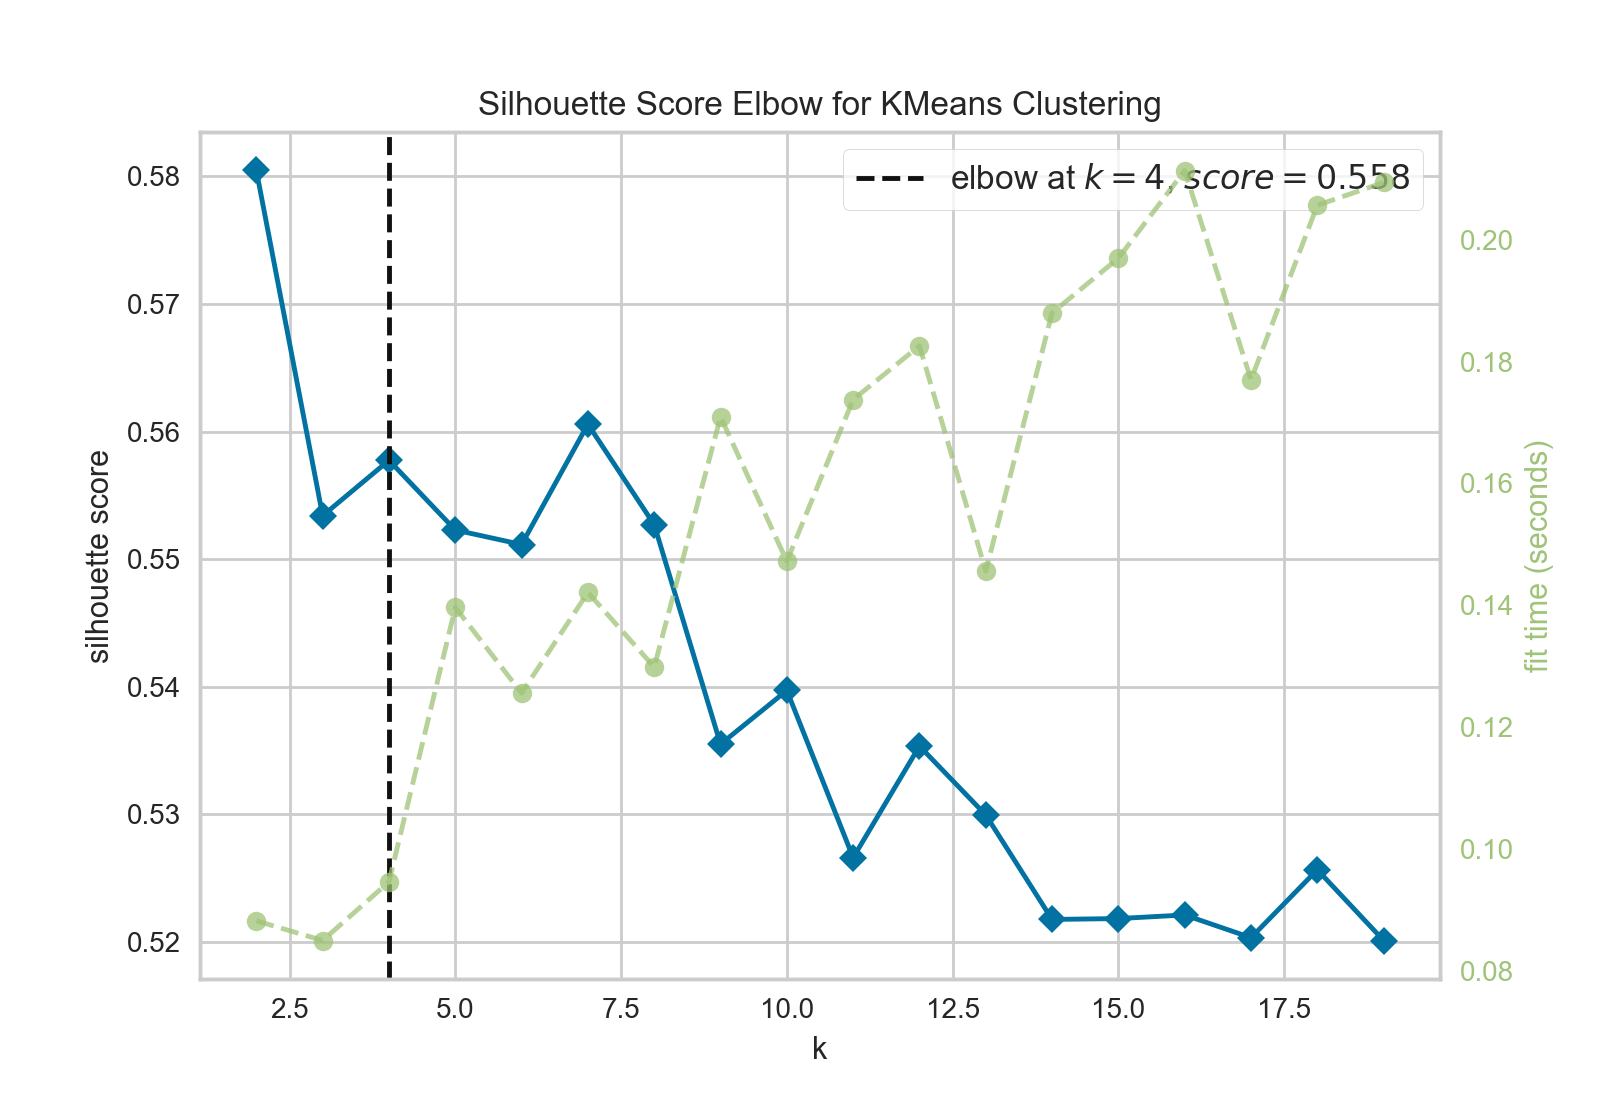
\includegraphics[width=.9\linewidth]{elbowds1.png}
        \caption{Timing curve vs silhouette coeff. dataset 1}\label{Fig:K-means vs silhouette coeff. dataset 1}
    \end{minipage}\hfill
    \begin{minipage}{0.5\textwidth}
        \centering
        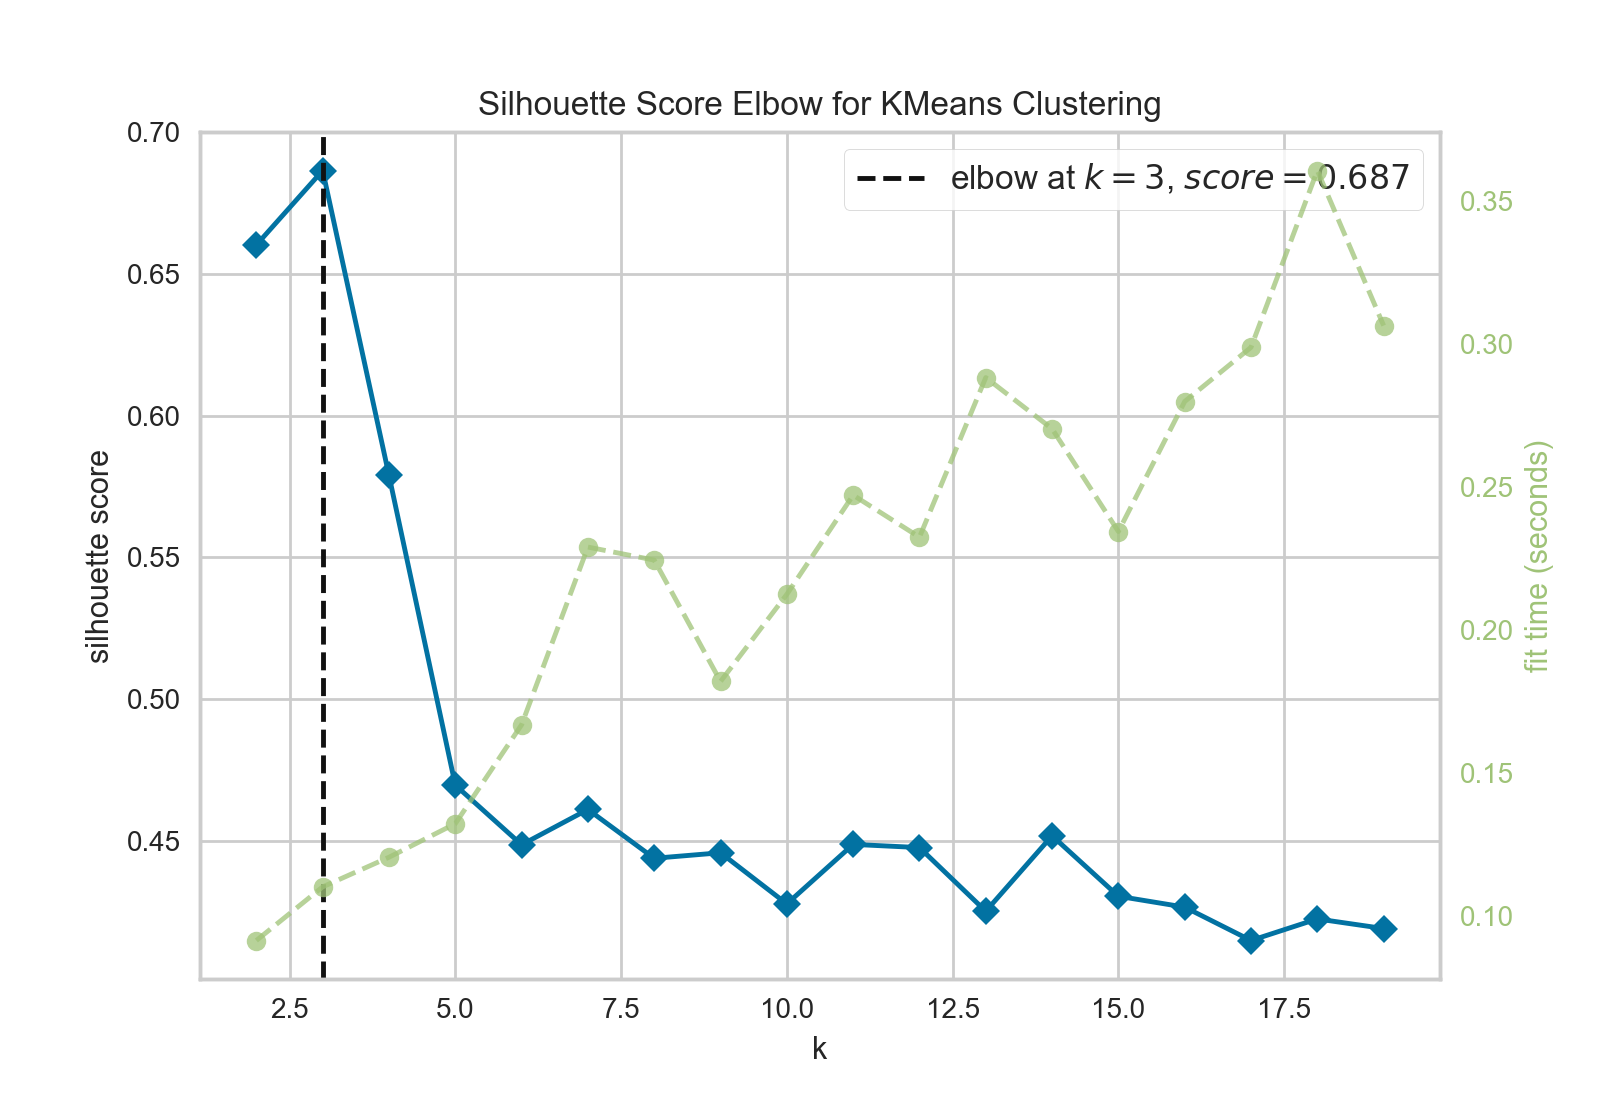
\includegraphics[width=.9\linewidth]{elbowds2.png}
        \caption{Timing curve vs silhouette coeff. dataset 2}\label{Fig:K-means vs silhouette coeff. dataset 2}
    \end{minipage}
\end{figure}
The two clustering techniques I explored for these datasets are K-Means clustering and Gaussian Mixture Models (Expectation Maximization)
In order to choose an appropriate $k$ to do k-means clustering, I used the elbow method\cite{developers_2020}.
Unless otherwise specified the standard distance measure I used was Euclidean distance.
Comparing all cluster cohesion metrics (mean distortion, silhouette coefficient, and Calinski-Harabasz score) here were
the elbow results:
\begin{center}
    \begin{tabular}{|c| c | c | c |}
        \hline
        & Metric                     & Cluster Count & Value \\
        \hline
        \hline
        Dataset 1 & Avg Silhouette Coefficient & 4             & 0.558 \\
        \hline
        Dataset 2 & Avg Silhouette Coefficient & 3             & 0.687 \\
        \hline
    \end{tabular}
\end{center}
Looking at figure~\ref{Fig:K-means vs silhouette coeff. dataset 1} and figure~\ref{Fig:K-means vs silhouette coeff. dataset 2} you can
see similar numbers in terms of the best "k".
I chose silhouette coeff over the other cluster cohesion metrics because it has a bias towards preferring well separated
clusters (coeffs closer to 1), which I anticipate would improve generalization and overall accuracy during a machine
learning process where the clusters are inputs to the learner.
Dataset 2 appears to have better separation between its 3 clusters than dataset 1's 4 clusters.
Doing further silhouette analysis on DS1 reveals that the clusters when plotted on it to the surface do not appear to
have a "cluster" round shape and instead are ovular, whereas data set two had similar characteristics to data set one
except that cluster two is actually interspersed in between cluster zero and cluster one, however this was only for the
first two features and others could have had better separation/shape.
Both clustering methods On both data sets appeared to have two very strongly defined clusters, and then up to two additional weakly defined clusters.
This more or less aligns with the fact that this is a binary classification problem and that samples could be placed into one of two clusters.
The clusters were more well defined and well separated on the second dataset which also makes sense given that all supervised learning methods performed better in terms of accuracy on this dataset relative to the first.
On closer inspection, the third and fourth clusters appear to be randomly dispersed throughout the dataset to capture outliers.
These clusters likely are noise capturers.
\begin{center}
    \begin{tabular}{|c| c | c | c |}
        \hline
        & Normalized Mutual Information & Homogeneity Score & Completeness Score \\
        \hline
        \hline
        Dataset 1 & 0.001                         & 0.002             & 0.001              \\
        \hline
        Dataset 2 & 0.189                         & 0.236             & 0.158              \\
        \hline
    \end{tabular}
\end{center}
Values closer to 1 are better than 0 in the above table for each score metric.
It seems that the performance of K-means is slightly better on dataset 2 than on 1.
To improve the performance of this we would likely need to include a dimensionality reduction technique, or modify the
dataset so that clusters are more hyper-spherical and separated from each other in the feature space.

\subsection{Expectation Maximization}\label{subsec:expectation-maximization}
\begin{figure}
    \begin{minipage}{0.5\textwidth}
        \centering
        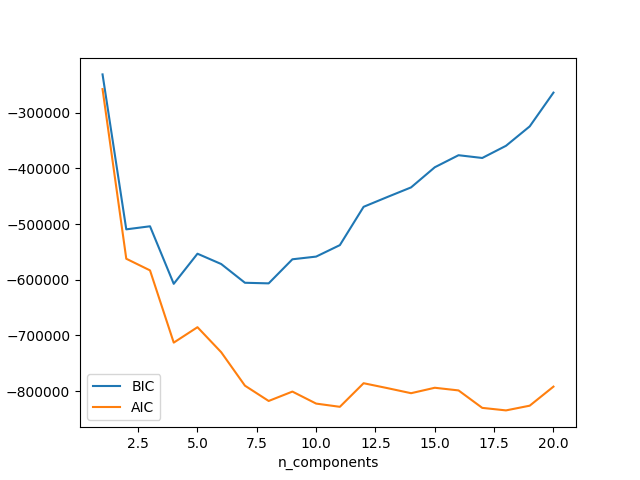
\includegraphics[width=.9\linewidth]{gmmcomponentsds1.png}
        \caption{n\_components vs AIC/BIC DS1}\label{Fig:GMM DS1}
    \end{minipage}\hfill
    \begin{minipage}{0.5\textwidth}
        \centering
        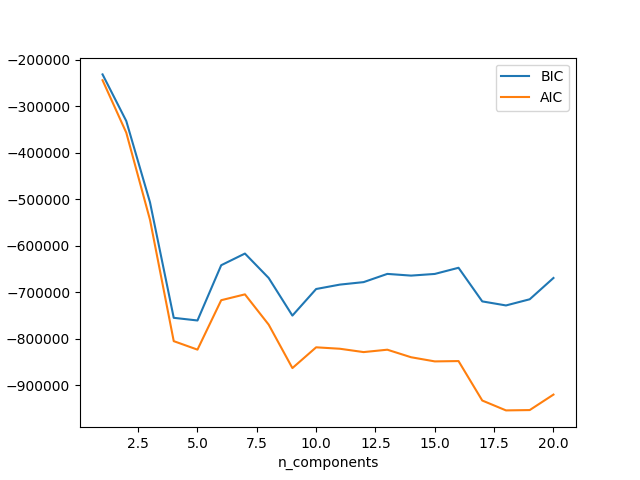
\includegraphics[width=.9\linewidth]{gmmcomponentsds2.png}
        \caption{n\_components vs AIC/BIC DS2}\label{Fig:GMM DS2}
    \end{minipage}
\end{figure}
For expectation maximization, I used the scikit-learn Gaussian mixture model function.
Based on my exploration I do not believe that the data are distributed in a hyper-spherical format, therefore a GMM would
be able to better group samples based on its ability to accommodate non-spherical hyper-surfaces.
In order to select a best value for the number of estimators in the model, I plotted the Bayesian Information Criterion
vs the Akaike Information Criterion, where they begin to diverge is likely the best place to stop in terms of n\_estimators.
In this case looking at figures~\ref{Fig:GMM DS1} and~\ref{Fig:GMM DS2} it appears to be the same as the optimal K found
previously (4 and 3 respectively.) After finding these and running best fits and comparing results I got:
\begin{center}
    \begin{tabular}{|c| c | c | c |}
        \hline
        & Normalized Mutual Information & Homogeneity Score & Completeness Score \\
        \hline
        \hline
        Dataset 1 & 0.002                         & 0.002             & 0.002              \\
        \hline
        Dataset 2 & 0.133                         & 0.174             & 0.108              \\
        \hline
    \end{tabular}
\end{center}
These clusters more or less make sense much in the same way that K-means did.
For dataset 1, GMM outperformed in terms of mutual information, homogeneity, and completeness shared by the clustering techniques and the actual labels
whereas for dataset 2 K-means outperformed, which indicates that the data was slightly more spherical than I anticipated.
However, neither of these clustering techniques did very well since all the values were close to 0 indicating that assigment
to clusters was independent and that the clusters themselves were not very independent, nor complete.



    \section{Dimensionality Reduction Discussion}\label{sec:dimensionality-reduction-discussion}

    In this section I explore four methods of dimensionality reduction on both of my datasets.

\subsection{Principal Components Analysis}\label{subsec:principal-components-analysis}
\begin{center}
    \begin{tabular}{|c| c |c|}
        \hline
        & Minimum Components to Explain 99.9\% Variance & Eigenvalues                               \\
        \hline
        \hline
        Dataset 1 & 2                                             & [11320901200.524, 54484006.504]           \\
        \hline
        Dataset 2 & 4                                             & [65088.565, 37527.175, 4525.986, 106.278] \\
        \hline
    \end{tabular}
\end{center}
Two features explain 100\% of the variance in the data in the case of PCA for dimensionality reduction, and four features explain
99.9\% of the variance in the case of the second dataset.
In the case of dataset one the eigenvalues are very large which would seem to imply that the data are close together and
the are being multiplied by a large number to separate.
Figures~\ref{Fig:PCA DS1} and~\ref{Fig:PCA DS2} show the projection of the transformed data according to their principal
components for the first two features (to allow for plotting).
\begin{figure}
    \begin{minipage}{0.5\textwidth}
        \centering
        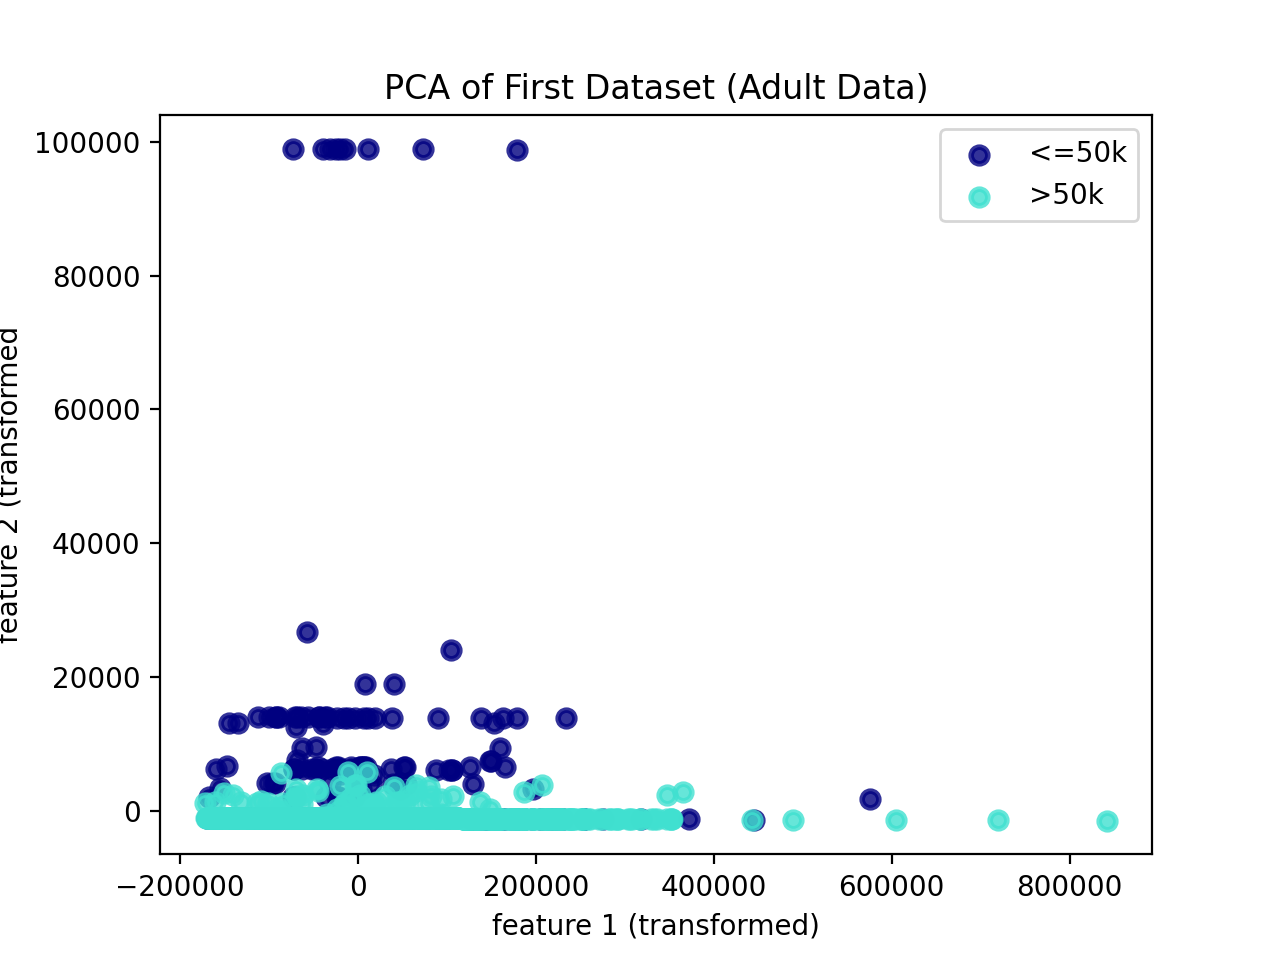
\includegraphics[width=.9\linewidth]{pcads1.png}
        \caption{DS1 Projection via PCA}\label{Fig:PCA DS1}
    \end{minipage}\hfill
    \begin{minipage}{0.5\textwidth}
        \centering
        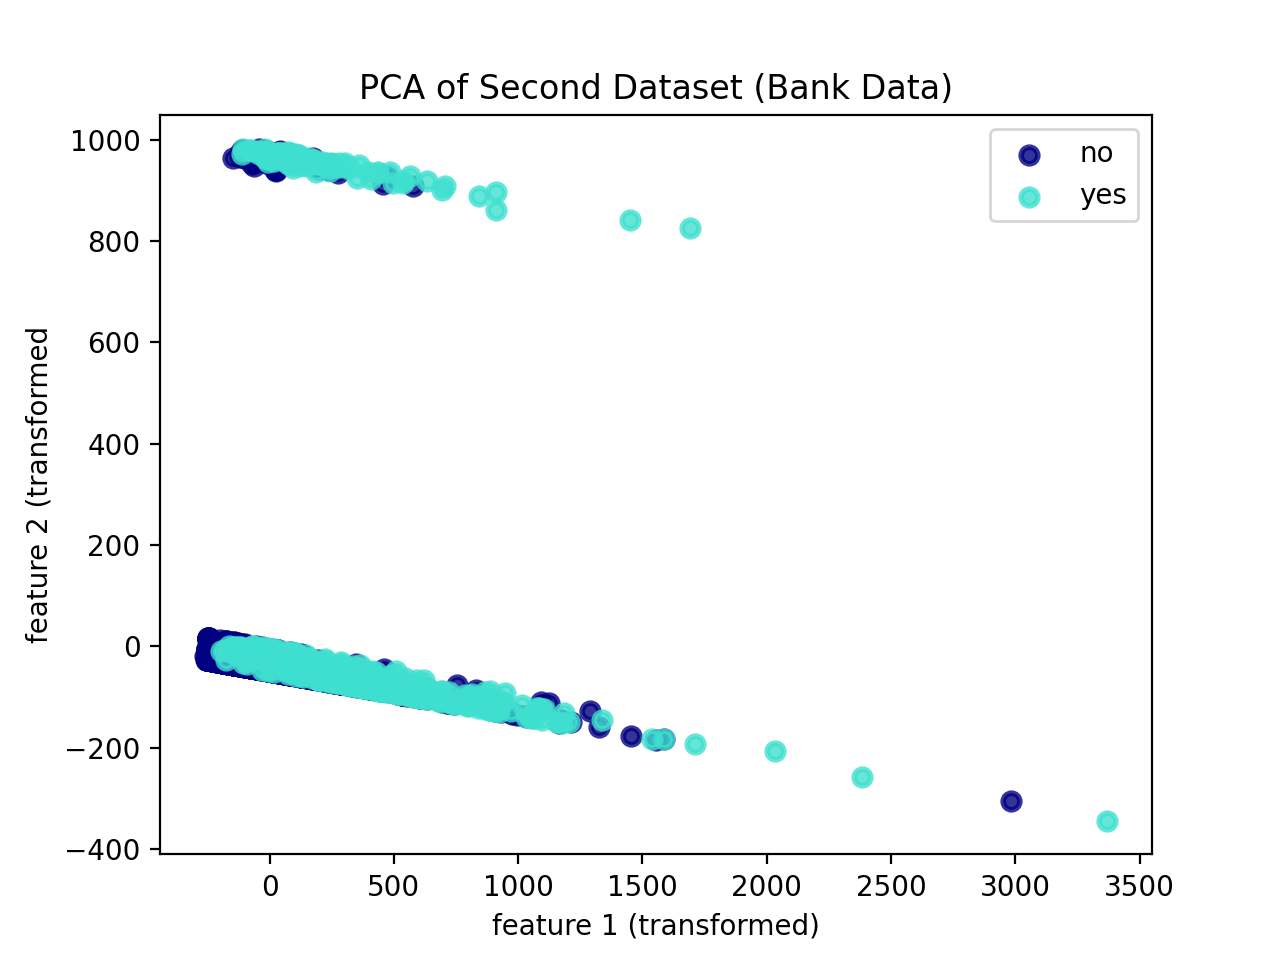
\includegraphics[width=.9\linewidth]{pcads2.png}
        \caption{DS1 Projection via PCA}\label{Fig:PCA DS2}
    \end{minipage}
\end{figure}

\subsection{Independent Components Analysis}\label{subsec:independent-components-analysis}
Similar to the previous I also attempted to search for the best number of components for each dataset.
According to Carsten Klein\cite{klein_2019}
"An interesting thing about two independent, non-Gaussian signals is that their sum is more Gaussian than any of the source signals.
Therefore we need to optimize W in a way that the resulting signals of Wx are as non-Gaussian as possible."
In other words, using a measurement like Kurtosis we can compare the "Gaussianity" of different ICA runs.
Since the normal distribution (Gaussian) has a kurtosis of 3, we are searching for ICA components with kurtosis of < 3.
In order to reduce the covariance of the feature vectors as much as possible (to in effect ensure they were independent
components, I elected to whiten the feature space before processing.)
Below is a table depicting the n-components selected for each dataset and the resulting Kurtosis.
\begin{itemize}
    \item For ICA, how kurtotic are the distributions?
    \item Do the projection axes for ICA seem to capture anything "meaningful"?
\end{itemize}
\begin{figure}
    \begin{minipage}{0.5\textwidth}
        \centering
        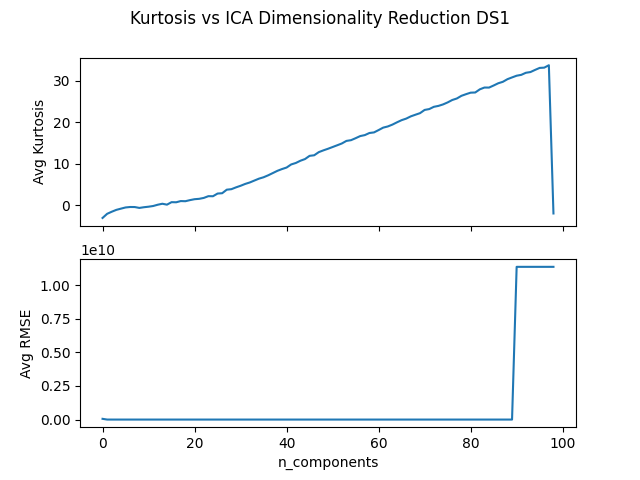
\includegraphics[width=.9\linewidth]{icads1.png}
        \caption{ICA Kurtosis vs RCError DS1}\label{Fig:ICA DS1}
    \end{minipage}\hfill
    \begin{minipage}{0.5\textwidth}
        \centering
        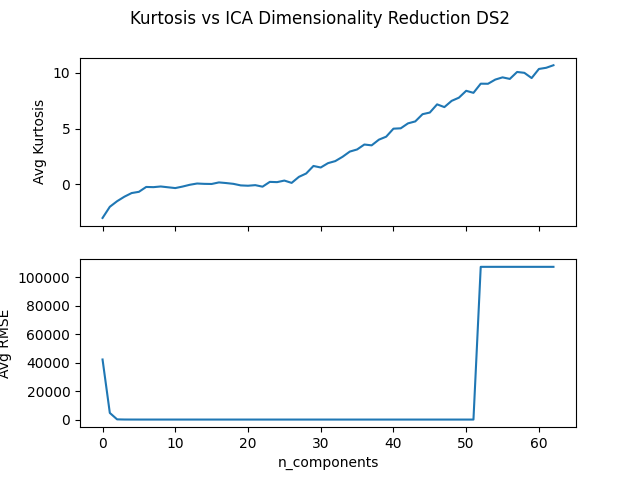
\includegraphics[width=.9\linewidth]{icads2.png}
        \caption{ICA Kurtosis vs RCError DS2}\label{Fig:ICA DS2}
    \end{minipage}
\end{figure}

\subsection{Randomized Projection}\label{subsec:randomized-projection}
\begin{itemize}

    \item Assuming you only generate k projections (i.e., you do dimensionality reduction), how well is the data reconstructed by the randomized projections? PCA?
    \item How much variation did you get when you re-ran your RP several times (I know I don't have to mention that you might want to run RP many times to see what happens, but I hope you forgive me)?
\end{itemize}
\begin{center}
    \begin{tabular}{|c| c |c|}
        \hline
        & Variance               & Standard Deviation \\
        \hline
        \hline
        Dataset 1 & 5.4456097845336664e+16 & 233358303.57057506 \\
        \hline
        Dataset 2 & 34540925361.18495      & 185851.89092711688 \\
        \hline
    \end{tabular}
\end{center}
\begin{figure}
    \begin{minipage}{0.5\textwidth}
        \centering
        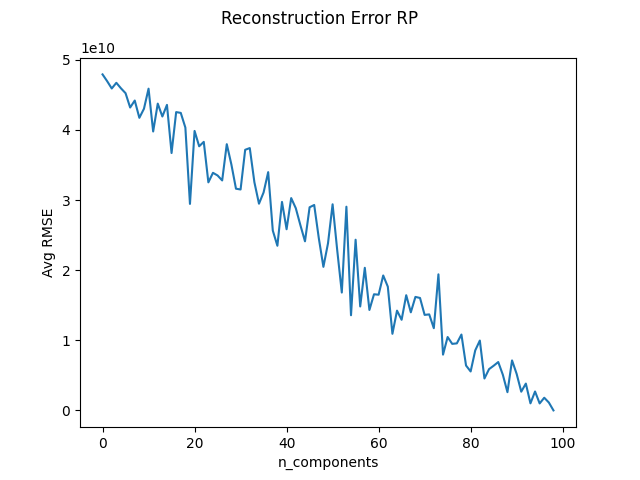
\includegraphics[width=.9\linewidth]{rpds1.png}
        \caption{RCError RP DS1}\label{Fig:RP DS1}
    \end{minipage}\hfill
    \begin{minipage}{0.5\textwidth}
        \centering
        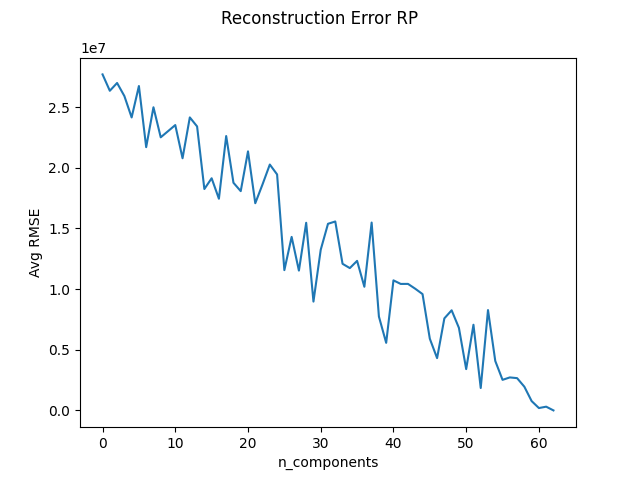
\includegraphics[width=.9\linewidth]{rpds2.png}
        \caption{RCError RP DS1}\label{Fig:RP DS2}
    \end{minipage}
\end{figure}

\subsection{Linear Discriminant Analysis}\label{subsec:linear-discriminant-analysis}
\begin{center}
    \begin{tabular}{|c| c |}
        \hline
        & Accuracy \\
        \hline
        \hline
        Dataset 1 & 82.86\%  \\
        \hline
        Dataset 2 & 91.17\%  \\
        \hline
    \end{tabular}
\end{center}


    \section{Clustering on Dimensionally Reduced Datasets}
    \begin{itemize}
        \item When you reproduced your clustering experiments on the datasets projected onto the new spaces created by ICA, PCA, and RP, did you get the same clusters as before? Different clusters? Why? Why not?
        \item When you re-ran your neural network algorithms were there any differences in performance? Speed? Anything at all?
    \end{itemize}

    \section{NN Learning on Clustered Datasets}

    \section{NN Learning on Clustered, Dimensionally Reduced Datasets}


    \bibliography{assignment3}
    \bibliographystyle{plain}
\end{document}